% ===================================================================
% Front matter — Full-bleed cover page (no margins)
% ===================================================================

\begin{titlepage}
\thispagestyle{empty}
% Full-bleed cover: image fills entire page including margins
\AddToShipoutPictureBG*{%
  \AtPageLowerLeft{%
    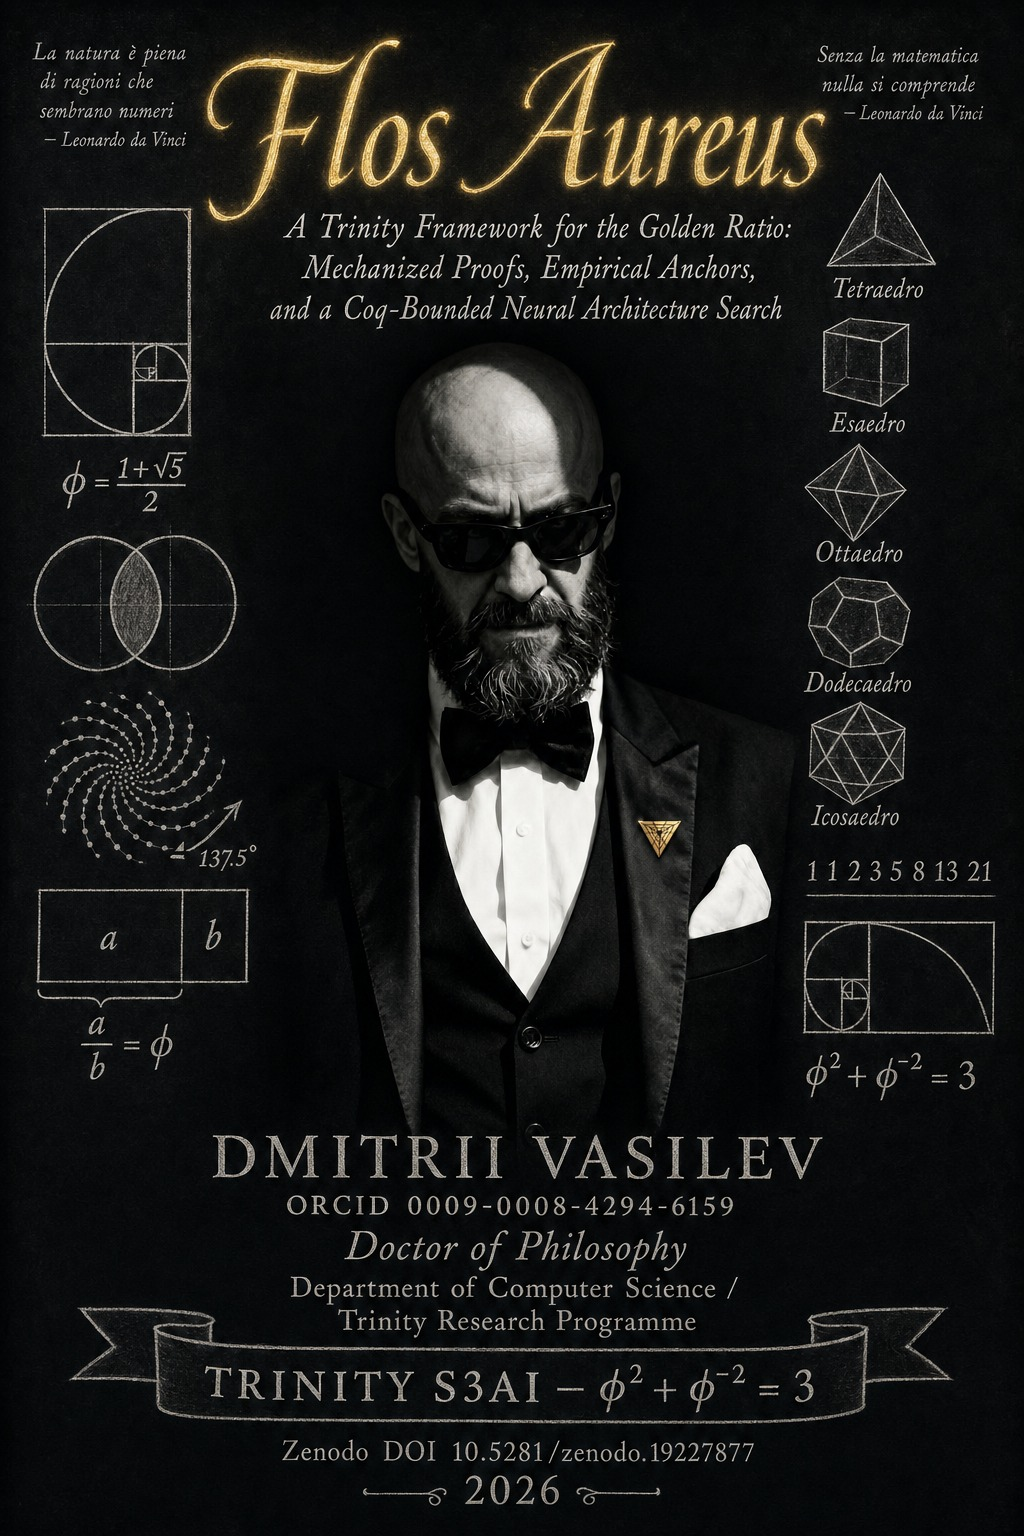
\includegraphics[width=\paperwidth,height=\paperheight,keepaspectratio=false]{assets/cover_v517.jpg}%
  }%
}
\mbox{}
\end{titlepage}

% ===================================================================
% Second page — title, author, ORCID, anchor (text moved here from cover)
% ===================================================================
\begin{titlepage}
\thispagestyle{empty}
\begin{center}

\vspace*{2cm}

{\LARGE\bfseries Flos Aureus}\\[0.4cm]
{\large\itshape A Trinity Framework for the Golden Ratio:\\
Mechanized Proofs, Empirical Anchors, and a Coq-Bounded\\
Neural Architecture Search}\\[1.2cm]

{\large Dmitrii Vasilev}\\[0.3cm]
{\small ORCID: \url{https://orcid.org/0009-0008-4294-6159}}\\[0.6cm]

\vfill

{\large A dissertation submitted in partial fulfilment\\
of the requirements for the degree of\\[0.3cm]
\textbf{Doctor of Philosophy}}\\[0.8cm]

{\normalsize Department of Computer Science}\\[0.1cm]
{\normalsize Trinity Research Programme}\\[0.6cm]

{\small Anchor identity:\quad $\varphi^{2} + \varphi^{-2} = 3$}\\[0.15cm]
{\footnotesize Zenodo DOI: \href{https://doi.org/10.5281/zenodo.19227877}{10.5281/zenodo.19227877}}\\[0.4cm]

{\small 2026}

\end{center}
\end{titlepage}
